\documentclass[thesis.tex]{subfiles}

\begin{document}

Now with the ability to calculate open-shell states, properties of and transitions between these states can be obtained.  In particular, this chapter focuses on beta-decay transitions between two particle-attached states and between two particle-removed states.  However, because these techniques are formulated in a general way, they can be applied to any type of one-body operator and any type of EOM-CC state.  First, this chapter describes beta-decay proccesses in detail and the relevant operators are introduced.  Then, these operators are used to construct effective coupled cluster operators that take important correlations from the ground-state wave function into account.  Finally, the effective operators are applied to EOM-CC states to calculate transition amplitudes for the corresponding processes.  These amplitudes can then be used to calculate observables like decay strengths and half-lives.

\section{Beta-Decay Properties} \label{section:betaproperties}

Nuclear beta decay describes a class of radioactive decays of the atomic nucleus that result as a consequence of the weak interaction.  These processes involve the exchange of a $\mathrm{W}$ boson which allows a quark within a proton or neutron to change type, thus converting a neutron to a proton or vice versa.  Additionally, this conversion is accompanied by an electron-antineutrino or positron-neutrino pair which ensures the process conserves charge and lepton number.  This work focuses on the three most common types of weak processes that occur within atomic nuclei: $\beta^{-}$ decay, $\beta^{+}$ decay, and electron capture (EC).  The first, $\beta^{-}$ decay, is the process whereby a down quark becomes an up quark, converting a neutron to a proton along with the creation of an electron, or $\beta^{-}$ particle, and an antineutrino.  Schematically, this decay can be written as,
\begin{equation*}
  \beta^{-}\ \text{decay}:  \hspace{0.5cm}  n\ &\longrightarrow\ p + e^{-} + \bar{\nu}_{e}.
\end{equation}
The corresponding mirror process is the $\beta^{+}$ decay, whereby an up quark becomes a down quark, converting a proton to a neutron with the creation of a positron, or $\beta^{+}$ particle, and a neutrino.  This decay is represented by,
\begin{equation*}
  \beta^{+}\ \text{decay}:  \hspace{0.5cm}   p\ &\longrightarrow\ n + e^{+} + \nu_{e}.
\end{equation}
A closely related process is the electron capture, whereby an atomic electron interacts with an up quark of a proton via a $\mathrm{W}$ boson, causing the conversion to a down quark and the release of a neutrino.  This process can be written as,
\begin{equation*}
  \text{Electron capture}:  \hspace{0.5cm}   p + e^{-}\ &\longrightarrow\ n + \nu_{e}.
\end{equation}
These three processes are schematically represented in Fig.\ \ref{fig:beta-0}.

\begin{figure}[h]
  \centering
  \begin{subfigure}{0.3333\linewidth}
    \centering
    \hspace{0.1cm}
    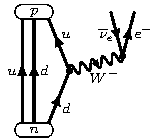
\includegraphics[height=3.5cm]{betadecay/BetaDecay-figure0.pdf}
    \caption{}
    \label{fig:beta-minus-0}
  \end{subfigure}
  \hspace{-0.05\linewidth}
  \begin{subfigure}{0.3333\linewidth}
    \centering
    \hspace{0.1cm}
    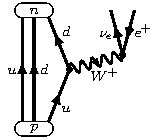
\includegraphics[height=3.5cm]{betadecay/BetaDecay-figure1.pdf}
    \caption{}
    \label{fig:beta-plus-0}
  \end{subfigure}
  \hspace{-0.05\linewidth}
  \begin{subfigure}{0.3333\linewidth}
    \centering
    \hspace{0.1cm}
    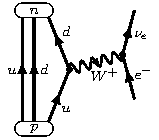
\includegraphics[height=3.5cm]{betadecay/BetaDecay-figure2.pdf}
    \caption{}
    \label{fig:beta-ec-0}
  \end{subfigure}
  \caption{Schematic representations of the three free-space weak processes in this work: $\beta^{-}$ decay (a), $\beta^{+}$ decay (b), and electron-capture (c).}
  \label{fig:beta-0}
\end{figure}


The \textit{Q-value} is a measure of the net energy of these processes.  In free space, only the $\beta^{-}$ decay has a positive Q-value and can occur spontaneously.  However, within a nucleus, correlations between nucleons cause the relatively simple, one-step exchanges in Fig.\ \ref{fig:beta-0} to take on more complicated, higer-order processes involving pion exchanges between different nucleons, see Fig.\ \ref{fig:beta-2}.  This also has the effect of changing the energetics of the $\beta^{+}$ decay and electron-capture processes such that their Q-values are positive and can occur within certain nuclei.  As a first approximation to these higher-order processes, it can be assumed that at the weak interaction occurs at very short length and time scales  due to the large mass of the $\mathrm{W}$ boson.  Known as the \textit{impulse approximation}, this treatment of beta-decay processes involves one nucleon as a spectator to the other nucleons, shown in Fig.\ \ref{fig:beta-1}.

\begin{figure}
  \centering
  \begin{subfigure}{0.3333\linewidth}
    \centering
    \hspace{0.1cm}
    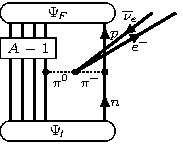
\includegraphics[height=3.5cm]{betadecay/BetaDecay-figure6.pdf}
    \caption{}
    \label{fig:beta-minus-2}
  \end{subfigure}
  \hspace{-0.05\linewidth}
  \begin{subfigure}{0.3333\linewidth}
    \centering
    \hspace{0.1cm}
    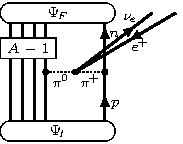
\includegraphics[height=3.5cm]{betadecay/BetaDecay-figure7.pdf}
    \caption{}
    \label{fig:beta-plus-2}
  \end{subfigure}
  \hspace{-0.05\linewidth}
  \begin{subfigure}{0.3333\linewidth}
    \centering
    \hspace{0.1cm}
    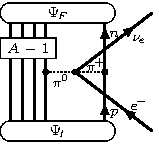
\includegraphics[height=3.5cm]{betadecay/BetaDecay-figure8.pdf}
    \caption{}
    \label{fig:beta-ec-2}
  \end{subfigure}
  \caption{Schematic representations of a higher-order weak interactions involving pion-exchange that occur within a nucleus, for $\beta^{-}$ decay (a), $\beta^{+}$ decay (b), and electron-capture (c).  These processes are not included in the impulse approximation.}
  \label{fig:beta-2}
\end{figure}

\begin{figure}
  \centering
  \begin{subfigure}{0.3333\linewidth}
    \centering
    \hspace{0.1cm}
    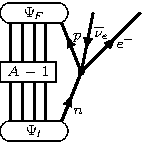
\includegraphics[height=3.5cm]{betadecay/BetaDecay-figure3.pdf}
    \caption{}
    \label{fig:beta-minus-1}
  \end{subfigure}
  \hspace{-0.05\linewidth}
  \begin{subfigure}{0.3333\linewidth}
    \centering
    \hspace{0.1cm}
    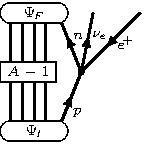
\includegraphics[height=3.5cm]{betadecay/BetaDecay-figure4.pdf}
    \caption{}
    \label{fig:beta-plus-1}
  \end{subfigure}
  \hspace{-0.05\linewidth}
  \begin{subfigure}{0.3333\linewidth}
    \centering
    \hspace{0.1cm}
    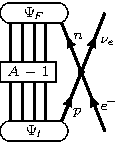
\includegraphics[height=3.5cm]{betadecay/BetaDecay-figure5.pdf}
    \caption{}
    \label{fig:beta-ec-1}
  \end{subfigure}
  \caption{Schematic representations of the impulse approximations to the different weak processes within an $A$-body nucleus: $\beta^{-}$ decay (a), $\beta^{+}$ decay (b), and electron-capture (c).  The active nucleon doesn't interact with the initial and final nuclei during the weak process. }
  \label{fig:beta-1}
\end{figure}

These beta-decay processes can be further characterized by the character of their angular momentum.  \textit{Allowed} beta decays involve an electron-antineutrino or positron-neutrino pair with no angular momenum, $L=0$.  In this case, there can be no parity change between the initial and final nuclear states.  Also, each pair spin-$\frac{1}{2}$ leptons carry a coupled spin of either $S=0$ or $S=1$.  Therefore, the initial and final nuclear states must have angular momenta that only differ by $0$ or $1$, ($\Delta J = 0, 1$).  Additionally, parity must be conserved for these interactions.  Transitions when the nuclear states are coupled to leptons with $S=0$ are known as \textit{Fermi transitions}, and transitions when the spin changes $S=1$ are known as \textit{Gamow-Teller transitions} (GT).  The summary of these selection rules are shown in table\ \ref{tab:beta-selection}.
\begin{table}
  \centering
  \begin{tabular}{ l @{\hskip 50pt} l @{\hskip 50pt} l } \hline
    \vspace{0.1mm} \\
    Decay Type     & $\Delta J = J_{F} - J_{I}$ & $\pi_{F}\pi_{I}$ \vspace{0.5mm} \\ \hline\hline
    \vspace{0.5mm} \\
    Fermi          & 0                         & +1 \\
    Gamow-Teller   & $1    (J_{F}=0\ \text{or}\ J_{I}=0)$   & +1 \\
    Gamow-Teller   & $0,1  (J_{F}>0\ \text{and}\ J_{I}>0)$  & +1 \vspace{1mm} \\ \hline
  \end{tabular}
  \caption{.}
  \label{tab:beta-selection}
\end{table}

The half-life of these processes $T_{1/2}$ can be calculated using a combination of both the Fermi and Gamow-Teller type transitions in the form of their reduced transition amplitudes, $B_{\text{F}}$ and $B_{\text{GT}}$, respectively.  These are measures of the overlap integral between the initial and final nuclear states for the different transitions and will be discussed in the next section.  Inserting these reduced transition amplitudes into the standard result from time-dependent perturbation theory gives the decay half-life,
\begin{equation}
  T_{1/2} = \frac{f}{K_{0}\left( B_{\text{F}} + B_{\text{GT}} \right)}.
\end{equation}
The factor $f$ represents a phase-space integral over the final nuclear and lepton states and depends on the decay Q-value.  The factor $K_{0}$ encodes the relevent constants involved,
\begin{equation}
  K_{0} = \frac{2\pi^{3}\hbar^{7}\ln 2}{m_{e}^{5}c^{4}G_{F}^{2}} \approx 6147 sec,
\end{equation}
where $m_{e}$ is the electron mass, and $G_{F}$ is the effective coupling constant of the impulse approximation.  The next section describes the process of using coupled cluster theory to include more correlations into this crude approximation.


\section{Coupled Cluster Effective Operators} \label{section:cc-operators}


The one-body beta-decay operators can be split into $\mathrm{hp}$, $\mathrm{hh}$, $\mathrm{pp}$, and $\mathrm{ph}$ components which are analagous to the one-body components of the effective Hamiltonian, see \ref{chapter:eff_ham_diagrams}.  The $\mathrm{hp}$ component has no connected terms in Eq.\ \eqref{}, and so it is unchanged by the similarity transformation,
\begin{align}
  \diagram{Eff_1b/Eff_1b-figure0} &= \diagram{Eff_1b/Eff_1b-figure1} \notag \\
  \oopint{\lambda}{i}{a} &= \opint{\lambda}{i}{a}.
\end{align}
The $\mathrm{pp}$ component is augmented by single excitations from the reference state.  This component's diagrammatic and algebraic expressions are,
\begin{align}
  \diagram{Eff_1b/Eff_1b-figure2} &= \diagram{Eff_1b/Eff_1b-figure3} + \diagram{Eff_1b/Eff_1b-figure4} \notag \\
  \oopint{\lambda}{a}{b} &= \opint{\lambda}{a}{b} - \sum\limits_{k}\oopint{\lambda}{k}{b}\tamp{a}{k}.
\end{align}
Similarly, the $\mathrm{hh}$ component is also augmented by single excitations from the reference state,
\begin{align}
  \diagram{Eff_1b/Eff_1b-figure5} &= \diagram{Eff_1b/Eff_1b-figure6} + \diagram{Eff_1b/Eff_1b-figure7} \notag \\
  \oopint{\lambda}{i}{j} &= \opint{\lambda}{i}{j} + \sum\limits_{c}\oopint{\lambda}{i}{c}\tamp{c}{j}.
\end{align}
The $\mathrm{ph}$ component of the effective beta-decay operator includes effects from single and double excitations from the reference state.  The diagrammatic and algebraic expressions for this component are,
\begin{align}
  \diagram{Eff_1b/Eff_1b-figure8} &= \diagram{Eff_1b/Eff_1b-figure9} + \diagram{Eff_1b/Eff_1b-figure10} + \diagram{Eff_1b/Eff_1b-figure11} + \diagram{Eff_1b/Eff_1b-figure12} \notag \\
  \oopint{\lambda}{a}{i} &= \opint{\lambda}{a}{i} + \sum\limits_{\mathclap{c}}\oopint{\lambda}{a}{c}\tamp{c}{i} - \sum\limits_{\mathclap{k}}\oopint{\lambda}{k}{i}\tamp{a}{k} + \sum\limits_{\mathclap{kc}}\oopint{\lambda}{k}{c}\tamp{ac}{ik}.
\end{align}

Like the higher-body interactions induced by the CC similarity transformation, two-body effective operators are induced from the one-body bare beta-decay operator.  Calculating properties using PA-EOM(2) and PR-EOM(2) states requires only two components of the effective two-body operator.  The $\mathrm{pphp}$ component is the results of double excitations from the reference state and is given by the following diagram and the corresponding expression,
\begin{align}
  \diagram{Eff_2b/Eff_2b-figure0} &= \diagram{Eff_2b/Eff_2b-figure1} \notag \\
  \oopint{\lambda}{ab}{ic} &= -\sum\limits_{k}\oopint{\lambda}{k}{c}\tamp{ab}{ik}.
\end{align}
Similarly, the $\mathrm{hphh}$ component is represented by the following diagram and its corresponding algebraic expression,
\begin{align}
  \diagram{Eff_2b/Eff_2b-figure2} &= \diagram{Eff_2b/Eff_2b-figure3} \notag \\
  \oopint{\lambda}{ia}{jk} &= \sum\limits_{c}\oopint{\lambda}{i}{c}\tamp{ca}{jk}.
\end{align}




\section{Calculating Beta-Decay Matrix Elements}

Fix these!!!!!!!
\begin{equation}
  \mathcal{M}_{\text{F}} \equiv \relement{\mathcal{F}}{\mathbf{\tau}}{\mathcal{I}} = \delta_{J_\mathcal{F}J_{\mathcal{I}}}\sum_{pq}\relement{p}{\mathbf{\hat{\tau}}}{q}\relement{\mathcal{F}}{\co{p}\ao{q}}{\mathcal{I}}
\end{equation}
\begin{equation}
  \mathcal{M}_{\text{GT}} \equiv \relement{\mathcal{F}}{\mathbf{\sigma\tau}}{\mathcal{I}} = \sum_{pq}\relement{p}{\mathbf{\hat{\sigma}\hat{\tau}}}{q}\relement{\mathcal{F}}{\co{p}\ao{q}}{\mathcal{I}}
\end{equation}

\begin{equation}
  \relement{p}{\mathbf{\hat{\tau}}}{q} = \delta_{n_{p}n_{q}}\delta_{l_{p}l_{q}}\delta_{j_{p}j_{q}}\delta_{t_{p}t_{q}\pm 1}\ \hat{j}_{p}
\end{equation}
\begin{equation}
  \relement{p}{\mathbf{\hat{\sigma}\hat{\tau}}}{q} = \sqrt{6}\ \delta_{n_{p}n_{q}}\delta_{l_{p}l_{q}}\delta_{t_{p}t_{q}\pm 1}\ \hat{j}_{p}\hat{j}_{q}\mathop{(-1)^{l_{p}+j_{p}+\frac{3}{2}}}\sixj{\frac{1}{2}}{\frac{1}{2}}{1}{j_{q}}{j_{p}}{l_{p}}
\end{equation}


\begin{equation}
  B_{\text{F}} \equiv \frac{g^{2}_{\text{V}}}{\hat{J}^{2}_{\mathcal{I}}}\lvert\mathcal{M}_{\text{F}}\rvert^{2}
\end{equation}
\begin{equation}
  B_{\text{F}} = \frac{g^{2}_{\text{V}}}{\hat{J}^{2}_{\mathcal{I}}}\sum_{\mathcal{F}\mathcal{I}}\frac{\element{\Lop^{\mathcal{I}}}{\mathbf{\tau}}{\Rop^{\mathcal{F}}}\element{\Lop^{\mathcal{F}}}{\mathbf{\tau}}{\Rop^{\mathcal{I}}}}{\braket{J_{\mathcal{I}}M_{\mathcal{I}};\lambda-\mu}{J_{\mathcal{F}}M_{\mathcal{F}}}^{2}}
\end{equation}


\begin{equation}
  B_{\text{GT}} \equiv \frac{g^{2}_{\text{A}}}{\hat{J}^{2}_{\mathcal{I}}}\lvert\mathcal{M}_{\text{GT}}\rvert^{2}
\end{equation}
\begin{equation}
  B_{\text{GT}} = \frac{g^{2}_{\text{A}}}{\hat{J}^{2}_{\mathcal{I}}}\sum_{\mathcal{F}\mathcal{I}}\frac{\element{\Lop^{\mathcal{I}}}{\mathbf{\sigma\tau}}{\Rop^{\mathcal{F}}}\element{\Lop^{\mathcal{F}}}{\mathbf{\sigma\tau}}{\Rop^{\mathcal{I}}}}{\braket{J_{\mathcal{I}}M_{\mathcal{I}};\lambda-\mu}{J_{\mathcal{F}}M_{\mathcal{F}}}^{2}}
\end{equation}


\begin{gather}
  B_{\beta^{-}} = \element{\Ref}{\Lop^{n}\mathop{(\mathbf{\hat{\beta^{-}}})^{\dagger}}\Rop^{p}}{\Ref}\element{\Ref}{\Lop^{p}\mathbf{\hat{\beta^{-}}}\Rop^{n}}{\Ref} \\
  B_{\beta^{-}} = \element{\Ref}{\Lop_{p}\mathop{(\mathbf{\hat{\beta^{-}}})^{\dagger}}\Rop_{n}}{\Ref}\element{\Ref}{\Lop_{n}\mathbf{\hat{\beta^{-}}}\Rop_{p}}{\Ref} \\
  B_{\beta^{-}} = \element{\Ref}{\Lop^{n}_{p}\mathop{(\mathbf{\hat{\beta^{-}}})^{\dagger}}\Rop_{0}}{\Ref}\element{\Ref}{\Lop_{0}\mathbf{\hat{\beta^{-}}}\Rop^{n}_{p}}{\Ref} \\
  B_{\beta^{-}} = \element{\Ref}{\Lop_{0}\mathop{(\mathbf{\hat{\beta^{-}}})^{\dagger}}\Rop^{p}_{n}}{\Ref}\element{\Ref}{\Lop^{p}_{n}\mathbf{\hat{\beta^{-}}}\Rop_{0}}{\Ref}
\end{gather}


\begin{gather}
  B_{\beta^{+}} = \element{\Ref}{\Lop^{p}\mathop{(\mathbf{\hat{\beta^{+}}})^{\dagger}}\Rop^{n}}{\Ref}\element{\Ref}{\Lop^{n}\mathbf{\hat{\beta^{+}}}\Rop^{p}}{\Ref} \\
  B_{\beta^{+}} = \element{\Ref}{\Lop_{n}\mathop{(\mathbf{\hat{\beta^{+}}})^{\dagger}}\Rop_{p}}{\Ref}\element{\Ref}{\Lop_{p}\mathbf{\hat{\beta^{+}}}\Rop_{n}}{\Ref} \\
  B_{\beta^{+}} = \element{\Ref}{\Lop^{p}_{n}\mathop{(\mathbf{\hat{\beta^{+}}})^{\dagger}}\Rop_{0}}{\Ref}\element{\Ref}{\Lop_{0}\mathbf{\hat{\beta^{+}}}\Rop^{p}_{n}}{\Ref} \\
  B_{\beta^{+}} = \element{\Ref}{\Lop_{0}\mathop{(\mathbf{\hat{\beta^{+}}})^{\dagger}}\Rop^{n}_{p}}{\Ref}\element{\Ref}{\Lop^{n}_{p}\mathbf{\hat{\beta^{+}}}\Rop_{0}}{\Ref}
\end{gather}


Quenching \cite{HARDY2005,TOWNER2008,KUBODERA1978,OSET1979}


\end{document}
